\subsubsection{Drehräder-Modell}
\begin{figure}[h!]
	\begin{subfigure}{.5\textwidth}
		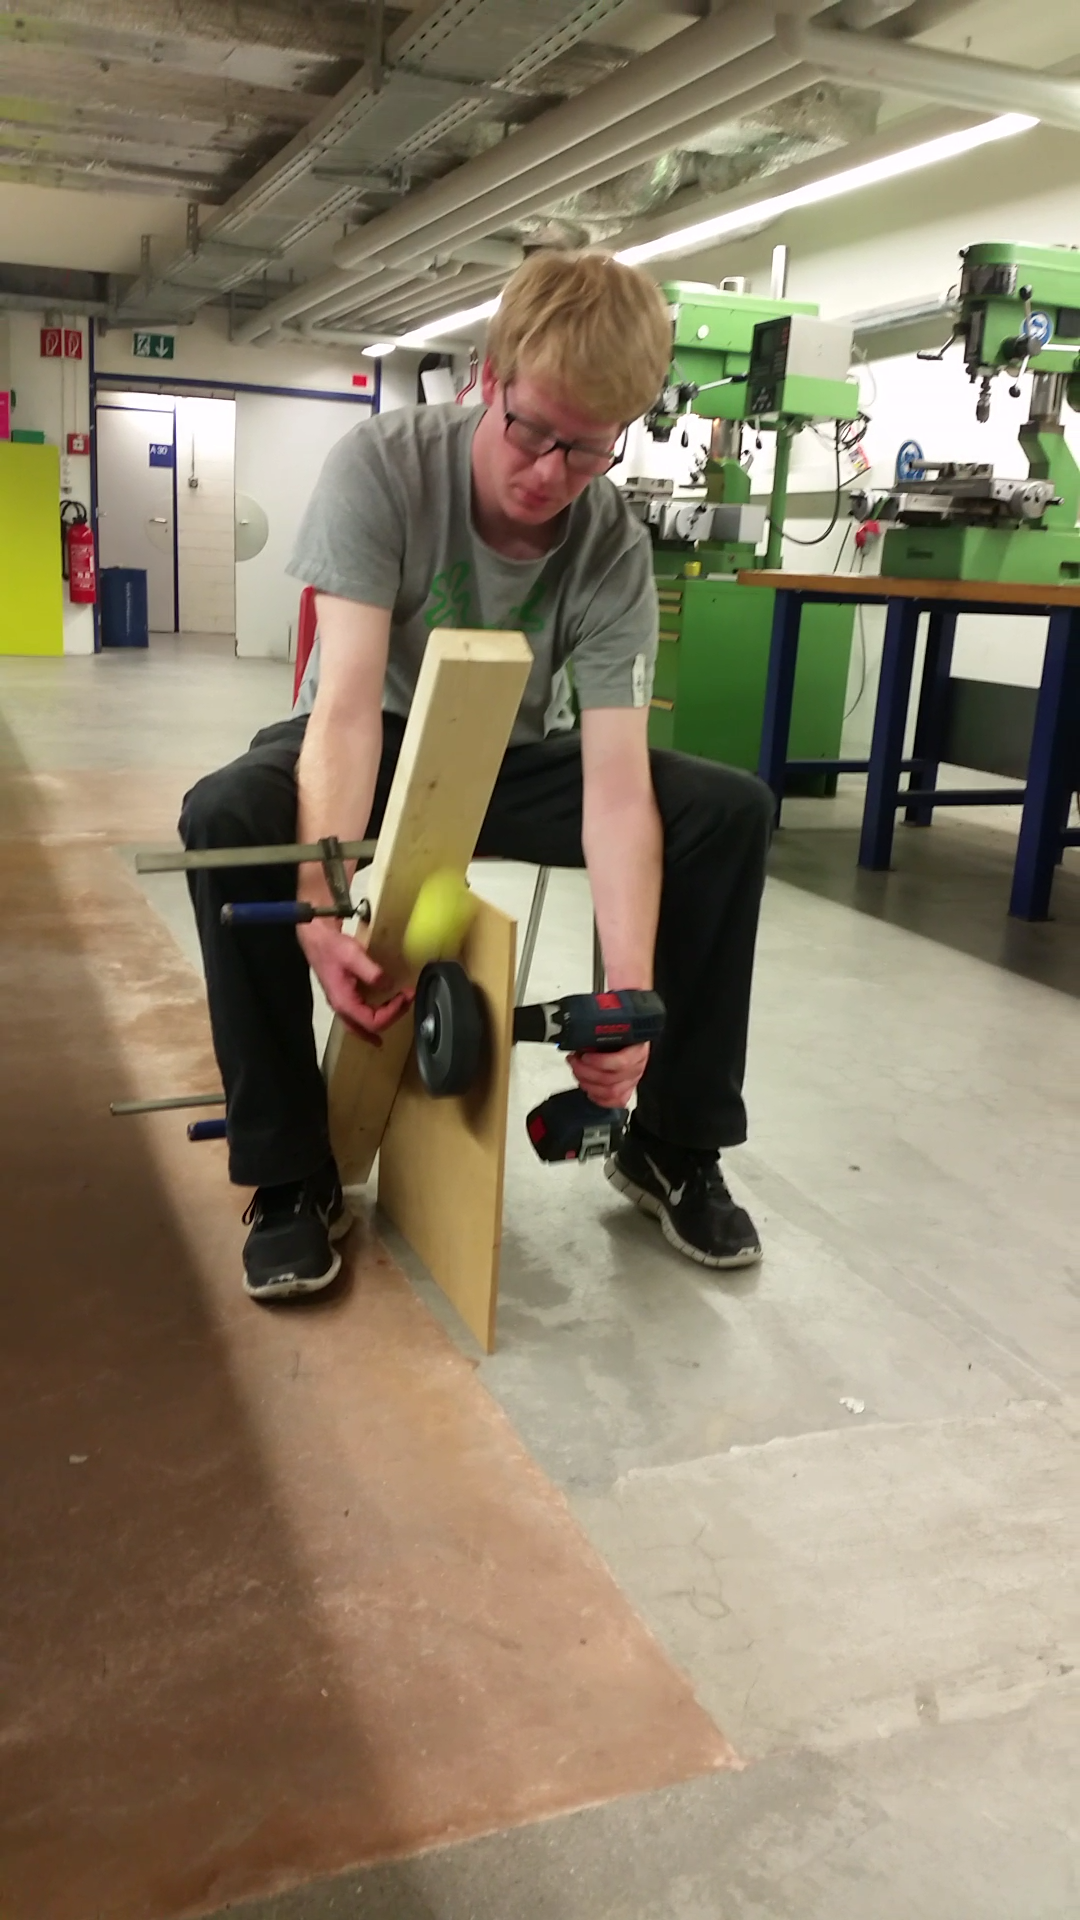
\includegraphics[width=1\textwidth]{../../fig/Versuch_Drehrad.png}
		\caption{Schrägen Wurf von der Seite}
		\label{fig:Aufbau der Versuch}
	\end{subfigure} %
	\begin{subfigure}{.5\textwidth}
		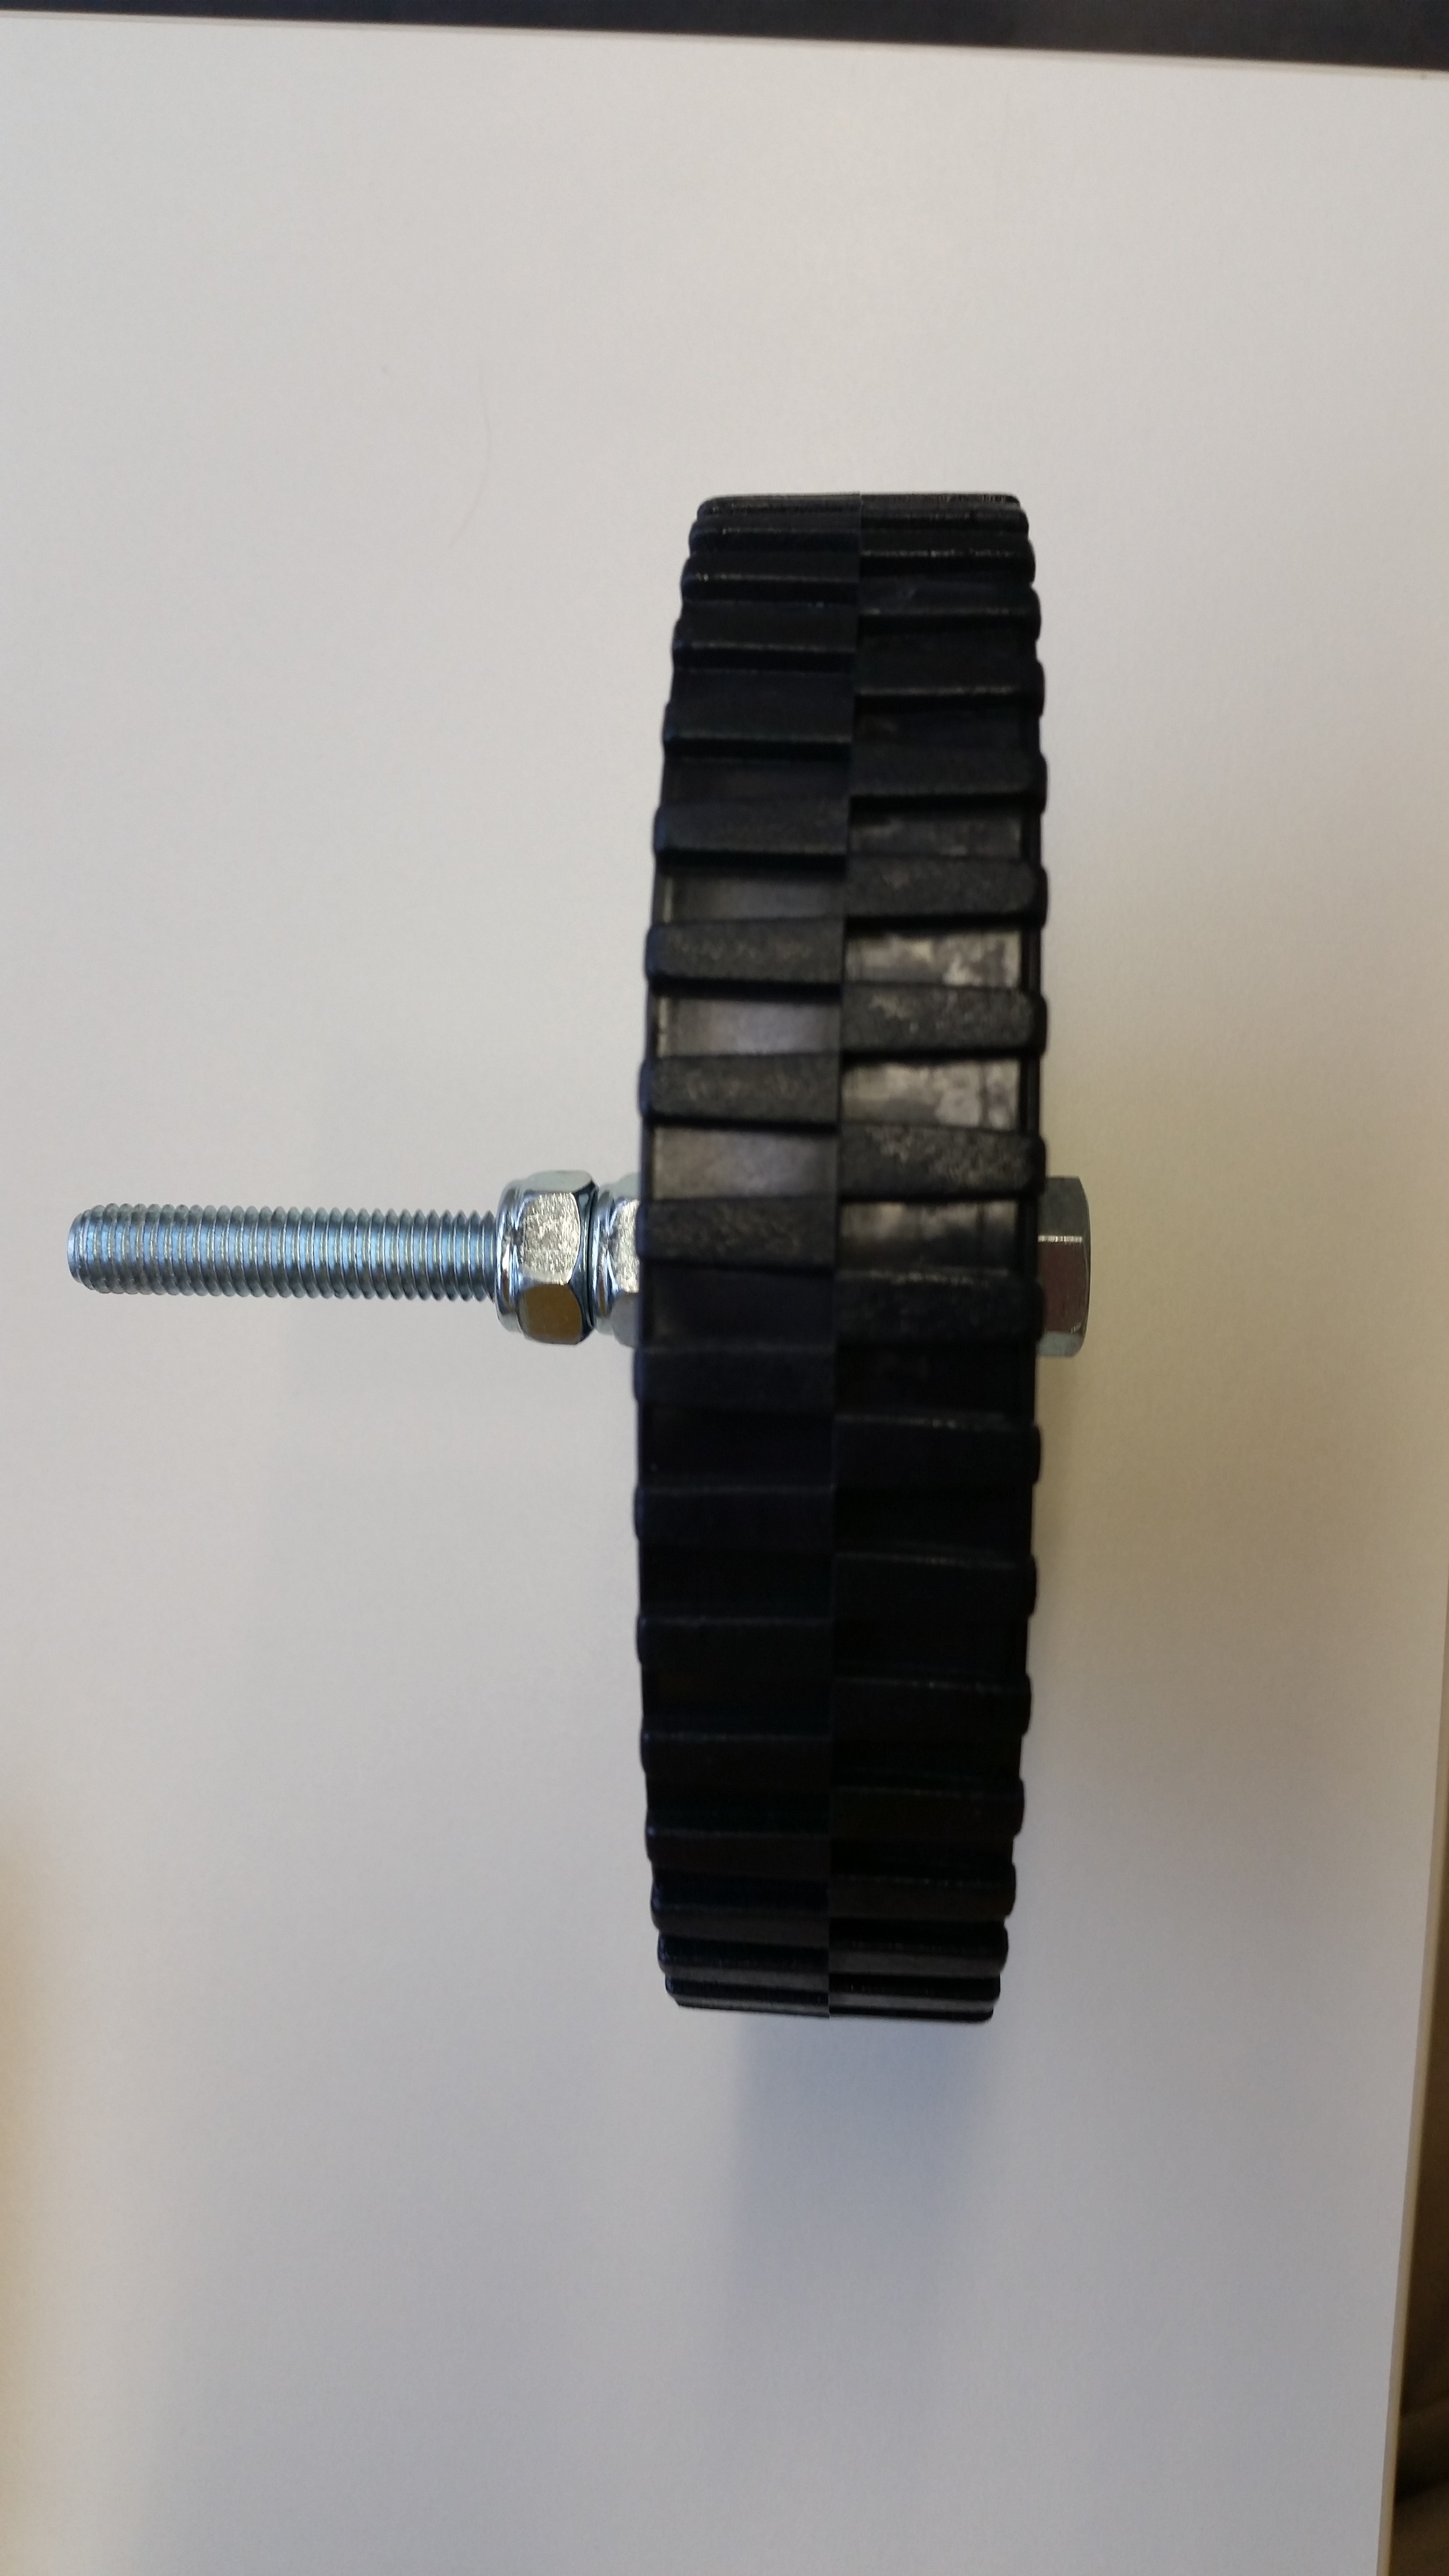
\includegraphics[width=1\textwidth]{../../fig/Drehrad_1.jpg}
		\caption{Schrägen Wurf von Oben}
		\label{fig:Drehrad}
	\end{subfigure}
	\caption{Berechnung der Schräger Wurf}
	\label{Drehrad Versuch}
\end{figure}
Wir haben einen 15 cm Durchmesser Drehrad aus PVC benutzt um einem Prototyp unseres Wurfmaschine zu Aufbauen. Als Betriebsmotor haben wir ein Akkubohrermaschine benutzt.
Mit ein kleines Aufbau haben wir versucht die Regelmässigkeit zu testen. Es war uns nicht wichtig ob die genaue Distanz erreicht wurde, sonst nur ob es bei jedem Schuss immer auf der selbe Abstand war. Mit der Versuch sollte auch nachgeschaut werden, was für eine Auswirkung der Drehung der Ball haben könnte. Der Versuch in 2 Arten gemacht: ein erstes mal mit der Drehrad oben der Ball, und ein zweites mit der Drehrad unten. Mit diesem Unterschied würde möglich die Auswirkung der Drehung der Ball zu festlegen und auch welche Vorrichtung einem besserem Schuss geben kann.\\
Nach mehrere versuche wurde festgelegt das es, auch mit ein groben Aufbau, dieses Wurfsystem sehr regelmässig ist. \\

